\paragraph{Dynamic Multicore Processor} DMPs contain hardware which can be modified post fabrication.
Mitall's survey ~\cite{MittalSurv2016} defines three types of modifiable resources: the core count~\cite{ipek2007CoreFusion}, number of resources that each core has~\cite{Homayoun3DPooling2012} and micro-architectural features~\cite{fallinhetblock2014,BauerRSE08,tavanaElastic}.
In our paper we focus on DMPs that modify the core count.

\paragraph{EDGE ISA} We assume a DMP similar to TFlex~\cite{kim2007tflex} using an Explicit Data Graph Execution~\cite{burger04edge} (EDGE) instruction set architecture (ISA).
EDGE ISAs encode dependencies between instructions at the ISA level.
Code is organised as blocks of instructions where all instruction communication is local to the block~\cite{smith2006edge}.
Each block has a single entry point but may have multiple exits.
This enables the architecture to dispatch blocks speculatively, with low overhead~\cite{putnam2010e2,kim2007tflex}, therefore, increasing exploitation of ILP.

 \begin{figure*}[t]
 \center
 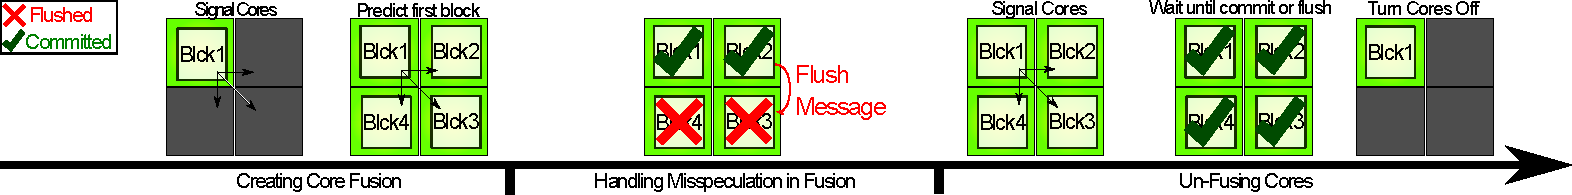
\includegraphics[width=1\textwidth]{cases-paper/graphics/background/proc_test.pdf}
\vspace*{-5mm}
 \caption{Core Fusion Mechanisms for our EDGE-based architecture.}\label{fig:dmp}
\vspace{-5mm}
 \end{figure*}
\paragraph{Core Fusion} 
Core Fusion is achieved by fusing a set of \textit{physical} cores to create larger \textit{logical} cores.
This does not modify the physical structure of the chip, instead it provides a unified view of a group of physical cores to the software.
For example, fusing two cores generates a logical core with twice the amount of execution units, register files and L1 cache.
Fusion is a dynamic modification and may occur during the execution of a program to better fit the workload.
Unlike traditional CMPs, fused cores will operate on the same thread and attempt to extract Instruction Level Parallelism (ILP) rather than Thread Level Parallelism (TLP)~\cite{micolet2016dmpstream,pricopi2012bahurupi}.
Figure~\ref{fig:dmp} shows the different stages and mechanisms of core fusion for a four core system.
When creating a new core fusion a master core informs all other cores about the fusion and sends the predicted next block address to the next available fused core.
When a core mis-predicts a branch in a fusion, it informs the other cores which flush any younger blocks.
When un-fusing, the master core informs the other cores, which then commit or flush their blocks and power down while the master core continues to fetch and execute blocks from the thread.
The extra hardware required to support dynamic reconfiguration is very minimal~\cite{kim2007tflex} since most of the machinery already in place can be reused such as the cache coherence protocol when fusing and un-fusing the cores.
We discuss this in further detail in Section~\ref{sec:setup}.
